\documentclass[a4paper]{article} 

%中文环境设置
\usepackage{xeCJK} 
\usepackage{indentfirst}
\setlength{\parindent}{2em}
\usepackage{enumitem}

\usepackage{abstract}
\renewcommand{\abstractname}{摘要}
\providecommand{\keywords}[1]{\textbf{\textit{关键词}} #1}

\setCJKmainfont{STSong} % 中文主字体设置 

\usepackage[colorlinks,linkcolor=blue, citecolor=blue]{hyperref}

% 常用宏包
\usepackage{float}
\usepackage{stfloats}
\usepackage{graphicx}
\usepackage{color}
\usepackage{supertabular}

% 代码环境设置
\usepackage{listings}
\lstset{
	columns=fullflexible,
 	frame=single,
 	breaklines=true,
}
\definecolor{lightgray}{gray}{0.9}
\newcommand{\inlinecode}[2]{\colorbox{lightgray}{\lstinline[language=#1]$#2$}}

% 页面段落设置
\usepackage{multicol}
\usepackage{geometry}
\geometry{left=3.18cm, right=3.18cm, top=2.54cm, bottom=2.54cm}
\linespread{1.3}
%\setlength{\parskip}{0.5em} 

% 数学环境设置
\usepackage{amsmath}
\usepackage{amssymb}
\usepackage{amsthm}
\usepackage{amsfonts}
\newtheorem{myDef}{Definition} 
\newtheorem{myThm}{Theorem}
\newtheorem{myProp}{Property}

\begin{document} 
\title{函数逼近与数据拟合\ 上机习题}
\author{吴佳龙 2018013418}
\date{}
\maketitle

\begin{abstract}
	结合理论分析和编程计算,运用不同方法求解了一函数的最佳平方逼近和近似最佳一致逼近。求解最佳平方逼近利用了Legendre 多项式,求解近似最佳一致逼近的两种方法分别为截断 Tchebychev 级数和插值余项极小化。
\end{abstract}

%\keywords{one, two, three, four}

\begin{multicols}{2}

\begin{section}{问题}

	设 $$f(x)=x^{2} \ln (2+x), x \in[-1,1]$$ 
	
	试求出权函数 $\rho(x)=1$ 的最佳平方逼近三次多项式。另外用 Tchebychev 截断级数的方法和插值余项极小化的方法分别给出近似最佳一致逼近三次多项式,并画图比较。

\end{section}

\begin{section}{最佳平方逼近}

	\begin{subsection}{算法原理}
		
		\begin{subsubsection}{法方程}
		
			设 $\left\{\varphi_{j}\right\}_{j=0}^{n} \subset L_{\rho}^{2}[a, b]$ 为线性无关函数,将最佳平方逼近函数表示为:$S_{n}^{*}(x)=\sum_{j=0}^{n} a_{j}^{*} \varphi_{j}(x)$,满足 $$\frac{\partial}{\partial a_{k}}(f-S_{n}^{*})=0 \Longrightarrow \sum_{j=0}^{n} a_{j}\left(\varphi_{j}, \varphi_{k}\right)=\left(f, \varphi_{k}\right)$$ 称为关于 $a$ 的法方程。
			
			若取 $\varphi$ 为正交多项式,则 Gram 矩阵成为对角阵,法方程易解。
			
		\end{subsubsection}

		\begin{subsubsection}{Legendre 多项式}
		
			Legendre 多项式 $$P_{n}(x)=\frac{1}{n ! 2^{n}} \frac{d^{n}}{d x^{n}}\left[\left(x^{2}-1\right)^{n}\right]$$ 是在区间 $[-1,1]$ 对应权函数 $\varphi(x) = 1$ 的正交多项式,满足:
			
			\begin{itemize}
				\item $\left(P_{n}, P_{m}\right) =\left\{\begin{array}{ll}{0,} & {n \neq m} \\ {\frac{2}{2 n+1},} & {n=m}\end{array}\right.$
				\item $(n+1) P_{n+1}(x)=(2 n+1) x P_{n}(x)-n P_{n-1}(x),\  n=0,1, \cdots $
			\end{itemize}
			
			由正交性和法方程,得 $ \alpha_{k}^{*}=\frac{\left(f, \varphi_{k}\right)}{\left(\varphi_{k}, \varphi_{k}\right)} $。具体地,将 Legendre 多项式归一化 $$\varphi_{n}(x)=\frac{1}{n ! 2^{n}} \sqrt{\frac{2 n+1}{2}} \frac{d^{n}}{d x^{n}}\left(x^{2}-1\right)^{n} $$ 得最佳平方逼近为 $$S_{n}^{*}(x)=\sum_{j=0}^{n} \alpha_{j}^{*} \varphi_{j}(x), \  \alpha_{j}^{*}=\int_{-1}^{1} f(x) \varphi_{j}(x) d x $$
			
		\end{subsubsection}
		
		\begin{subsubsection}{误差}
			
			误差 $\delta_{n}=f-S_{n}^{*}$ 满足 $$\left(f, S_{n}^{*}\right)=\left(S_{n}^{*}, S_{n}^{*}\right) \Longrightarrow\left\|\delta_{n}\right\|_{2}^{2}=(f, f)-\left(S_{n}^{*}, S_{n}^{*}\right)$$
			
		\end{subsubsection}
		
	\end{subsection}
	
	\begin{subsection}{算法实现}
	
		用 Legendre 多项式求最佳平方逼近的 MATLAB 实现如下:
		
\begin{lstlisting}[language=Matlab]
function coeff = myLegendreSquareApprox(f)
% 用Legendre多项式求最佳平方三次逼近
% 返回值 coeff 为 (1,4) 的向量,分别表示从常数项到三次项的系数

% 归一化的 Legendre 多项式
P0 = @(x)(sqrt(1/2));
P1 = @(x)(sqrt(3/2).*x);
P2 = @(x)(sqrt(5/8)*3.*(x.^2-1/3));
P3 = @(x)(sqrt(7/8).*x.*(5*x.^2-3));

a0 = integral(@(x)(f(x).*P0(x)),-1,1);
a1 = integral(@(x)(f(x).*P1(x)),-1,1);
a2 = integral(@(x)(f(x).*P2(x)),-1,1);
a3 = integral(@(x)(f(x).*P3(x)),-1,1);

coeff = [sqrt(1/2)*a0-sqrt(5/8)*a2, sqrt(3/2)*a1-3*sqrt(7/8)*a3, 3*sqrt(5/8)*a2, 5*sqrt(7/8)*a3];
end


\end{lstlisting}
		
	\end{subsection}
	
	\begin{subsection}{计算结果}
		
		计算得最佳平方逼近:
		
		\begin{equation} \nonumber
			\begin{aligned} S_3^{leg}(x)&=0.554258x^3+0.572954x^2\\ &-0.012249x+0.012489 \end{aligned}	
		\end{equation}
		
		并得到 $$\left\|f-S_3^{leg}\right\|_2 = 0.016549$$ $$\left\|f-S_3^{leg}\right\|_{\infty} = 0.043434$$
	\end{subsection}
	
\end{section}

\begin{section}{近似最佳一致逼近:截断 Tchebychev 级数近似}

	\begin{subsection}{算法原理}
	
		\begin{subsubsection}{Tchebychev 多项式}
		
			Tchebychev 多项式 $$T_{n}(x)=\cos (n \arccos x)$$ 是在 $[-1,1]$ 上对应权函数 $\rho(x)=\frac{1}{\sqrt{1-x^{2}}}$ 的正交多项式,满足:
			
			\begin{itemize}
				\item $\left(T_{n}, T_{m}\right)=\left\{\begin{array}{ll}{0,} & {n \neq m} \\ {\frac{\pi}{2},} & {n=m \neq 0} \\ {\pi,} & {n=m=0}\end{array}\right.$
				\item $T_{n+1}=2 x T_{n}-T_{n-1}$
				\item 在 $(-1,1)$ 上有 $n$ 个不同的零点 $x_{k}=\cos \frac{2 k-1}{2 n} \pi, k=1, \cdots, n$
				\item 在 $(-1,1)$ 上有 $n+1$ 个极值点 $x_{k}^{*}=\cos \frac{k}{n} \pi, k=0, \cdots, n$
			\end{itemize}
			
		\end{subsubsection}
		
		\begin{subsubsection}{截断 Tchebychev 级数}
			
			$f$ 对应 Tchebychev 多项式展开的广义 Fourier 级数(Tchebychev 级数)为 $$f \sim \frac{c_{0}}{2}+\sum_{k=1}^{+\infty} c_{k} T_{k}(x), \ c_{k}=\frac{2}{\pi} \int_{-1}^{1} \frac{f(x) T_{k}(x)}{\sqrt{1-x^{2}}} d x$$
			
			取前 $n+1$ 项部分和 $$S_{n}^{*}(x)=\frac{c_{0}}{2}+\sum_{k=1}^{n} c_{k} T_{k}(x)$$ 对于 $f \in C^{(r)}[-1,1](r \geq 2)$ 计算可得 $$f(x)-S_{n}^{*}(x)=c_{n+1} T_{n+1}(x)+\mathcal{O}\left(\frac{1}{(n+1)^{r-1}}\right)$$
			
			而 $T_{n+1}(x)$ 恰有 $n+2$ 个轮流为 $\pm 1$ 的极值点,根据 Tchebychev 定理,$S_{n}^{*}$ 可以作为 $f$ 的近似最佳一致逼近多项式。
			
		\end{subsubsection}
		
	\end{subsection}
	
	\begin{subsection}{算法实现}
		
		用截断 Tchebychev 级数的方法近似最佳一致逼近多项式的 MATLAB 实现如下:
		
\begin{lstlisting}[language=Matlab]
function coeff = myTchebychevUniformApprox(f)
% 截断 Tchebychev 级数近似最佳一致三次逼近
% 返回值 coeff 为 (1,4) 的向量,分别表示从常数项到三次项的系数

% Tchebychev 多项式
T0 = @(x)(1);
T1 = @(x)(x);
T2 = @(x)(2*x.^2-1);
T3 = @(x)(4*x.^3-3.*x);

c0 = 2/pi*integral(@(x)(f(x).*T0(x)./sqrt(1-x.^2)),-1,1);
c1 = 2/pi*integral(@(x)(f(x).*T1(x)./sqrt(1-x.^2)),-1,1);
c2 = 2/pi*integral(@(x)(f(x).*T2(x)./sqrt(1-x.^2)),-1,1);
c3 = 2/pi*integral(@(x)(f(x).*T3(x)./sqrt(1-x.^2)),-1,1);

coeff = [c0/2 - c2, c1-3*c3, 2*c2, 4*c3];
end
\end{lstlisting}
		
	\end{subsection}
	
	\begin{subsection}{计算结果}
		
		计算得近似最佳一致逼近:
		
		\begin{equation} \nonumber
			\begin{aligned} S_3^{tche}(x)&=0.562101x^3+0.550725x^2\\&-0.016446x+0.018594 \end{aligned}	
		\end{equation}
		
		并得到偏差 $$\left\|f-S_3^{tche}\right\|_{\infty} = 0.023663$$

	\end{subsection}
	
\end{section}


\begin{section}{近似最佳一致逼近:Lagrange 插值余项极小化}
	
	\begin{subsection}{算法原理}
	
		在 $x_{1}, \cdots, x_{n}$ 上插值,由插值余项公式:$$\left\|R_{n-1}\right\|_{\infty} \leq \frac{M_{n}}{n !}\left\|\omega_{n}\right\|_{\infty}, \ M_{n}=\left\|f^{(n)}\right\|_{\infty}$$
		
		由于 $2^{1-n} T_{n}(x)$ 是 $[-1,1]$ 上模最小的首一多项式,极小化 $\left\|\omega_{n} \right\|_{\infty}$,也就是令 $\omega_{n}(x)=2^{1-n} T_{n}(x)$,也就是取 $$x_{k}=\cos \frac{2 k-1}{2 n} \pi$$ 为插值节点。
		
		这样有 $$\left\|R_{n-1}\right\|_{\infty} \leq \frac{M_{n}}{n !2^{n-1}}$$ 且余项近似有轮流为正负的偏差点,可看做 $f$ 的近似最佳一致逼近。
		
	\end{subsection}
	
	\begin{subsection}{算法实现}
	
		用Lagrange 插值余项极小化的方法近似最佳一致逼近多项式的 MATLAB 实现如下:
		
\begin{lstlisting}[language=Matlab]
function coeff = myLagrangeUniformApprox(f)
% 插值余项极小化 近似最佳一致三次逼近
% 返回值 coeff 为 (1,4) 的向量,分别表示从常数项到三次项的系数

n = 4;
% Tchebychev 多项式零点
x = cos((2*(1:n)-1)/2/n*pi);
coeff = myLagrangeInterp(x, f(x));
end
\end{lstlisting}
	
		Lagrange 插值的实现可参见插值法的实验报告。
		
	\end{subsection}
	
	\begin{subsection}{计算结果}
	
		计算得近似最佳一致逼近:
		
		\begin{equation} \nonumber
			\begin{aligned} S_3^{lag}(x)&=0.548141x^3+0.552144x^2\\&-0.006136x+0.017918 \end{aligned}	
		\end{equation}
		
		并得到偏差 $$\left\|f-S_3^{lag}\right\|_{\infty} = 0.028058$$
		
	\end{subsection}
	
\end{section}

\begin{section}{方法比较}
	
	\begin{subsection}{图像}
	
		将 $f,\ S_3^{leg}(x),\ S_3^{tche}(x),\ S_3^{lag}(x)$ 的图像作出,如图 \ref{plot} 所示。
		
		可以看到,三种方法的得到的逼近多项式都与原函数十分接近。
		
		\begin{figure*}[ht] %h默认参数是可以浮动,不是固定在当前位置。如果要不浮动,你就可以使用大写float宏包的H参数,固定图片在当前位置,禁止浮动。
			\centering %使图片居中显示
			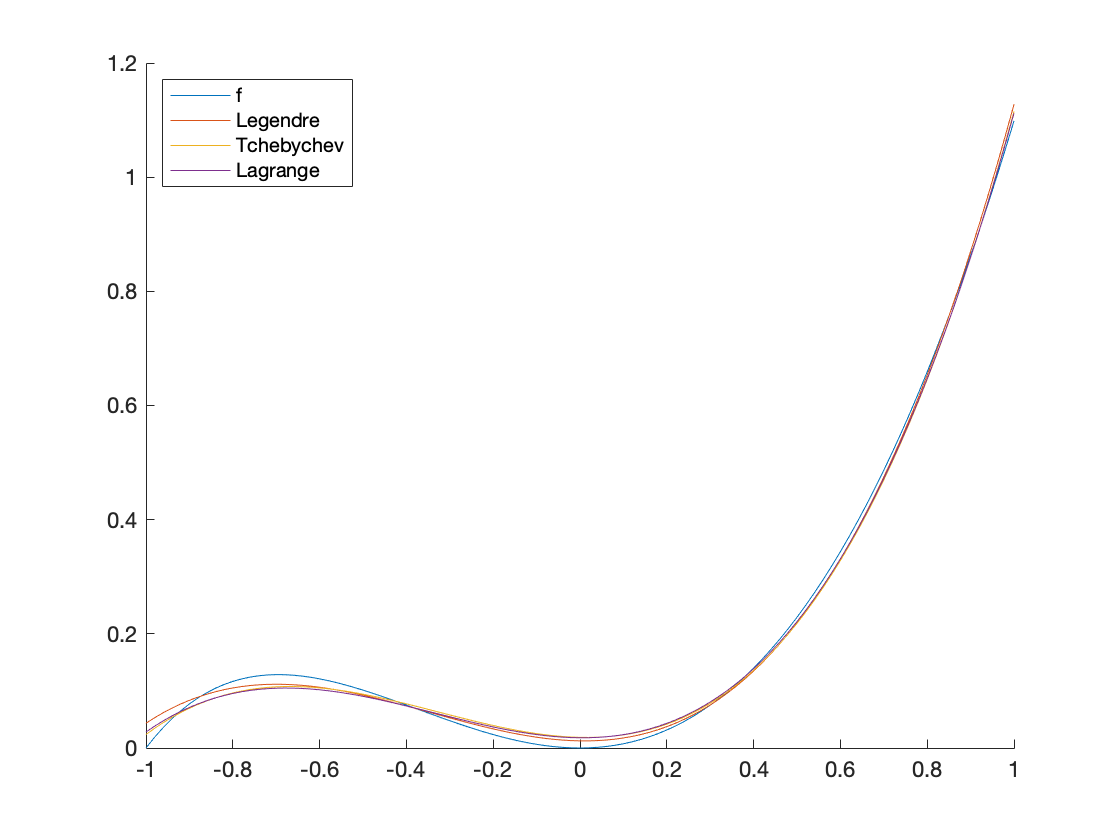
\includegraphics[width = 0.9\textwidth]{img/plot.png} 
			\caption{图像}
			\label{plot} 
		\end{figure*}	
		
	\end{subsection}
	
	\begin{subsection}{误差}
	
		将 $S_3^{leg}(x),\ S_3^{tche}(x),\ S_3^{lag}(x)$ 的误差作出,如图 \ref{error} 所示。
		
		\begin{table}[H]
		\begin{tabular}{c|c|c|c}
		\hline
		                         & $S_3^{leg}(x)$ & $S_3^{tche}(x)$ & $S_3^{lag}(x)$ \\ \hline
		$\left\|f-S_3\right\|_2$ & 0.043434       & 0.023663        & 0.028058      
		\end{tabular}
		\caption{偏差}
		\end{table}
		
		\begin{figure*}[ht] %h默认参数是可以浮动,不是固定在当前位置。如果要不浮动,你就可以使用大写float宏包的H参数,固定图片在当前位置,禁止浮动。
			\centering %使图片居中显示
			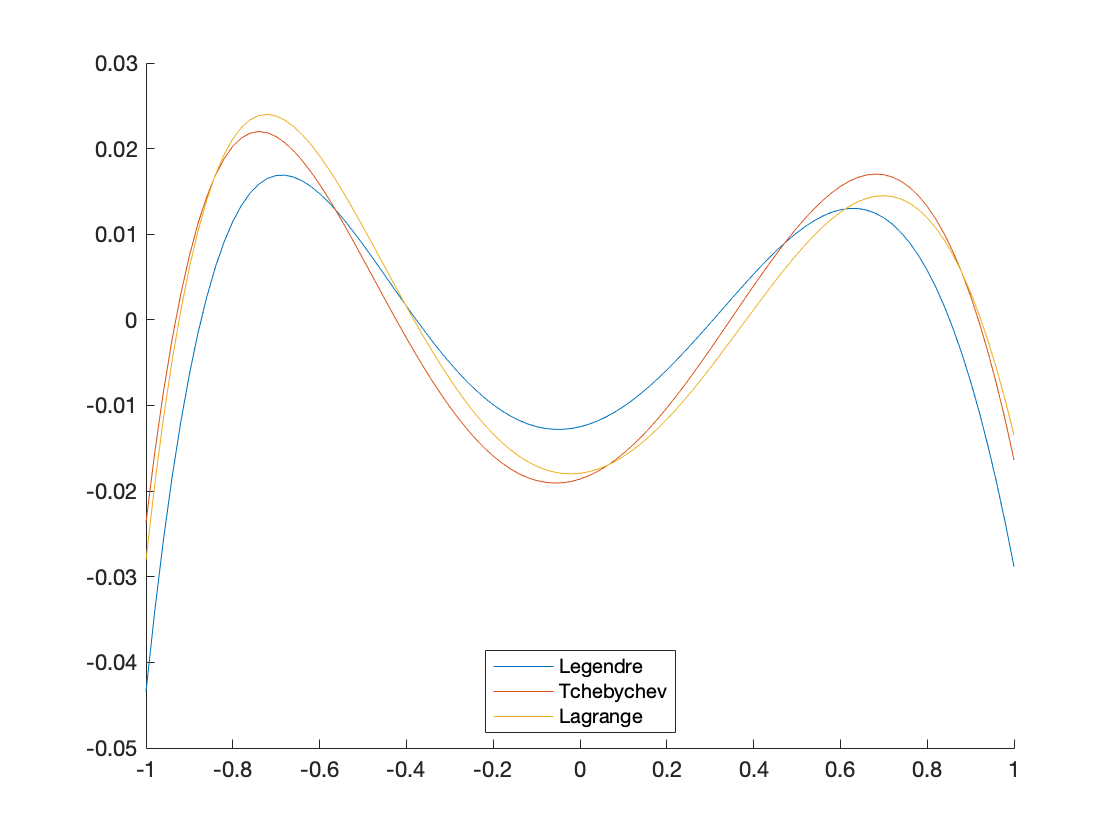
\includegraphics[width = 0.9\textwidth]{img/error.png} 
			\caption{误差}
			\label{error} 
		\end{figure*}
		
		可以看到,近似最佳一致逼近 $S_3^{tche}(x),\ S_3^{lag}(x)$ 都有五个近似的偏差点,偏差比 $S_3^{leg}(x)$ 较小。
		
	\end{subsection}

	
\end{section}
	
\begin{section}{总结}
	
	本次实验对于求解最佳平方逼近和近似最佳一致逼近的方法进行了理论分析和编程计算,作出图像并比较 了它们的结果。
	
	计算结果符合预期,观察到近似最佳一致逼近的五个近似的偏差点,加深了对正交多项式以及 Tchebychev 定理等的理解。
	
\end{section}

\end{multicols}

%\bibliographystyle{unsrt}
%\bibliography{ref.bib}

%\begin{thebibliography}{99}    %参考文献开始
%	\bibitem{ml}周志华. 机器学习[M]. 清华大学出版社, 2016.   
%\end{thebibliography}	

\end{document}

